\documentclass[conference]{IEEEtran}
\ifCLASSINFOpdf

\else

\fi
\usepackage{graphicx}
\hyphenation{op-tical net-works semi-conduc-tor}


\begin{document}
%
% paper title
% can use linebreaks \\ within to get better formatting as desired
% Do not put math or special symbols in the title.
\title{Mapping the Surface Mines using Unmanned Aerial Vehicles}
% author names and affiliations
% use a multiple column layout for up to three different
% affiliations
\author{\IEEEauthorblockN{Srikanth Malla}
\IEEEauthorblockA{B.Tech, VIT University,\\ Vellore, 632014,\\ India\\
Email: malla.srikanth2012@vit.ac.in}
\and
\IEEEauthorblockN{Chaitanya Malla}
\IEEEauthorblockA{B.Tech, VNIT,\\ Nagpur, 440010,\\ India\\
Email: chaitanyamalla1993@gmail.com}}


% make the title area
\maketitle

\begin{abstract}
Advances in robotics in minings helps to survey a mine and produce accurate 3d model. They are creating an economical impact by cutting down the huge costs involved in surveying the Surface Mines. In this paper we present a method to perform a survey with Unmanned Aerial Vehicles (UAV) for both the open cast and open pit mines using low cost photogrammetry techniques.
(can add one more line about project)
\end{abstract}
\section{Introduction}
Surface mining is a huge earth moving activity on this planet which needs a lot of planning activities, that are performed in various stages. Precision is the key for this planning and improves the efficiency. Aerial view of landscapes helps the project to plan the activities accurately and also in its design.\\
Aerial photogrammetry is used during early exploration stage to identify the untouched geography of the desired location. With the help of the obtained aerial footages an efficient planning And design of the mine can be made. The locations of railway tracks, bridges, lakes, flowing rivers,  location of vegetation etc can be identified and this helps a lot in the mine planning. The distances and directions of this important or sensitive spots can be identified and according to this, the location of stockpiles, dump heaps, drainages and sumps, tailing ponds, recovery units, bunkers can be put properly in our mine plan.\\
Next to this  the aerial photography is also being used in mine operations in these days.
As the mining activities occurs in hectares of land, the monitoring of these activities is a difficult task. But doing this surveillance activity with the conventional aerial survey method is very expensive. So here comes the unmanned aerial vehicles to do the risk free and economical surveillance of the daily mining activities in surface mines.  
As the  UAVs fly in low altitude the precision of ground models obtain is very high. With the help of image processing technology and by using structure from motion concept this became an alternative for the LIDAR Technology by producing more accurate and precise output.\\
Images with higher resolution are captured with the cameras attached to the drones and these images are processed in software to obtain Digital surface model and Digital Terrain model.
These drones can be operated by a pilot or they can move on their own with autonomous flight controlling techniques. This even reduces the efforts of drone pilots.\\
\section{Methodology}
We are using quadrotor uav for the inspection of the surface mines because of its agility, maneuverability, simplistic mechanical design.\\   
Here we have 4 degrees of freedom by our coverage planning algorithm, which are position of the quadrotor $<x, y, z, yaw>$.where yaw is to get the information at what angle the photo is taken and x,y,z is to get the info from where the photo is taken.\\
Whereas the roll and pitch  are not needed for the coverage algorithm but it is needed to controlled for the motion.\\
\subsection{Planning Algorithm}
We assume we have a partial idea of how the inspection area (3d model) looks like, mostly it is oriented in xy plane. Here we use STL file where the 3d Model contains triangular facets with normals describing their orientation. 
STL file is sliced using planes parallel to xz or yz. By intersecting the 3d  model with the planes, we obtain intersection points, they intersection points are\\ 
This becomes a travelling salesman problem all the waypoints \\
Let’s say we have waypoint set $X={x_i \mid 0<i<n+1}$ where n is no of waypoints. \\
Travelling salesman problem formulation:\\
\begin{equation} \label{eq:8}
\sum_{i=1}^{n}\sum_{j=1,j\neq i}^{n}\mid\mid x_i-x_j\mid\mid_2c_{ij}
\end{equation}\\
where\\
$c_{ij}$ is 1 if path goes from waypoint i to j, else 0
\begin{equation} \label{eq:8}
\sum_{i=1,i\neq j}^{n}x_{ij}=1; j=1,...,n
\end{equation}\\
\begin{equation} \label{eq:8}
\sum_{j=1,j\neq 1}^{n}x_{ij}=1; i=1,...,n
\end{equation}\\
But solving tsp problem is computationally expensive, which is impossible for this application as the number of waypoints are very large. So, we move on to very simplistic algorithm (greedy planner) \\
Greedy planner:\\
Euclidean distance (because it is open area without obstacles)\\
\begin{equation} \label{eq:8}
Eudist(x_i)=\mid\mid x_i-rp\mid\mid_2
\end{equation}\\
Choose the waypoint 
\begin{equation} \label{eq:8}
x^*=arg_{x_i}min{Eudist(x_i)}
\end{equation}\\
When the waypoint is reached 
\begin{equation} \label{eq:8}
\mid\mid x^*-rp\mid\mid_2 < threshold \Rightarrow X-{x*}
\end{equation}\\
This continues until 
\begin{equation} \label{eq:8}
X=\{\}
\end{equation}\\
This planner performance mostly depends on the initial or starting position of the robot. It gives near overall optimal path.\\
\\
Structure from Motion (sfm) (obtaining 3d information from 2d images):\\
Humans perceive  3D structure in their environment just by moving through it. When the observer is moving the object around the observer also moves, thus information is obtained from the images that are sensed over time.\\
Obtaining structure from the motion is  similar to finding structure from stereo vision[ ]. In both the cases, the correspondence between images and the reconstruction of 3D object needs to be done.\\
We are using photoscan pro software for the 3D model reconstruction of the 3d model (specify the format) which uses above described method\\
From the obtain DTM and DSM models the volumes of stockpiles and dump heaps are generated by using point cloud technology which creates three dimensional view of the bodies.-(point clouds: Point clouds are the set of point consisting the 3Dimensional $<x,y,z>$ coordinates for each points, usually used to represent the surface of the bodies. Laser scanners output these formats. These are also created from stereo image to get 3D structure from the 2D images.)
\\
From the obtained volumes, calculations goes as-

\subsection{In mining operations}
Percentage of ore is know from feasibility reports X\%. X tons of ore in 100 tons of total excavated material. The volume of excavated dump is calculated with UAV methods which is some Y. Multiplying the volume Y with density of waste/nonprofit material gives the number of tons of waste excavated. Even by using other calculations we can find the amount of dump from the obtained volume. Then we can cross check it to the amount of ore that should be obtained from the excavated waste. It is always less than the estimated X\% in real because of errors and losses of ore into the waste. But if it is very far away from the expected correction factor then examination of the errors has to be made to know the faults in the operations. In this way rectification in the operational activities can be made by assessing reports and plans to get the desired targets of production.

\subsection{For stock piles}
The stockpiles are generally heaps of the excavated ore which is stored openly. The volumes of these stockpiles are calculated with the UAVs then the mass can be obtained by density of the material. As the mass should be constant and  we even  know the actual mass that we excavated, it can be confirmed that the changes happen here will be in volume and density. But if we cross check it with calculated mass from volume obtained this gives error that means the quality of stockpile is changing. The customer needs a particular quality value and with time the quality changes because of weather conditions and oxidation etc., So with this alert a plan can be made either to sell the stock fast or to take care of its quality. During summers the outer part of the heap will be dry and moist free in hot regions and during rainy the moisture content increases a lot. If the heap is of metal content then reactions take place which results in changing the percentages and quality. This can even be observed to an extent in aerial images from the colour changes of the heaps because of its reactions like oxidations. 

\subsection{In Mine planning}
From the obtained aerial footages of high resolution and by using point cloud generation a 3D model of the mine with total number of benches, contour and everything that can be seen is produced. A realistic virtual model can be simulated. By using some softwares and giving the rock properties, soil conditions, groundwater conditions and faults etc, we can produce a real time model which shows us the chances of bench failures that are likely to happen with change in time, change in weather and rock properties. This helps a lot in safety planning activities. It gives a probability of failure in advance that may lead to accident, which can be controlled with preventive measures.
\section{Implementation}
The whole setup is implemented on a Iris plus quadrotor, equipped with 2 dimensional brushless motors gimbal (for camera stabilization) and Gopro Hero4 Camera (to get high resolution photos ). For the pose-estimate we are using GPS sensor and the waypoints are transformed into GPS coordinates before inspection. 
\begin{figure}[h]
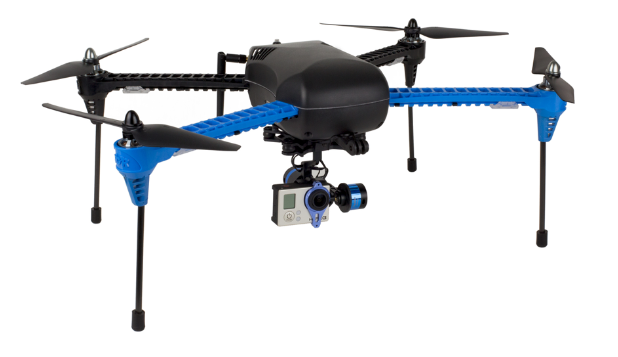
\includegraphics[width=6cm]{iris.png}
\centering
\caption{ Iris plus equipped with gopro and GPS sensor}
\label{iris_img}
\end{figure}

\section{Results}
\section{Conclusion}
we can extend it to simulate the vehicle accidents, road slippages and sump overflow etc, With this obtained predictions one can assess the future problems in advance and preventive measures can be taken in prior to avoid the risks. A graphic interface image can be created to show the life of the mine with the present excavation methods and how this life of mine changes by changing different parameters and factors governing. 
\begin{thebibliography}{1}

\bibitem{}

Eisenbeiss, Henri. \emph{A mini unmanned aerial vehicle (UAV): system overview and image acquisition.} International Archives of Photogrammetry. Remote Sensing and Spatial Information Sciences 36.5/W1 (2004).
\bibitem{}
Siebert, Sebastian, and Jochen Teizer. \emph{Mobile 3D mapping for surveying earthwork projects using an Unmanned Aerial Vehicle (UAV) system.} Automation in Construction 41 (2014): 1-14.
\bibitem{}
Nex, Francesco, and Fabio Remondino. \emph{UAV for 3D mapping applications: a review.} Applied Geomatics 6.1 (2014): 1-15.
\bibitem{}
Paterson, J. O. 2007. Accuracy Assessment of Unmanned Aerial Vehicle (UAV) – Borne Photogrammetry for Volume Estimations in Mining Applications. Hons. diss., Curtin University of Technology. 
\bibitem{}
Henri Eisenbeiss., and Li Zhang., 2006: Comparison of DSMs generated from mini UAV imagery and terrestrial laser scanner in a cultural heritage application. IAPRS Volume XXXVI, Part 5, Dresden 25-27 September 2006.
\bibitem{}
Allan Chikwanha, Sibonelo Motepe and Riaan Stopforth, \emph{Survey and requirements for search and rescue ground and air vehicles for mining applications}, 19th International Conference on Mechatronics and Machine Vision in Practice (M2VIP), 28-30th Nov 2012, Auckland, New-Zealand.
\bibitem{}
Bae, K-H., D. Belton and D. D. Lichti. 2007. Pre-processing Procedures for Raw Point Clouds from Terrestrial Laser Scanners. Journal of Spatial Science 52(2): 41-50. 

\end{thebibliography}


\end{document}